%\documentclass[11pt]{report}



%\begin{document}

\chapter{Technical overview}
%\addcontentsline{toc}{chapter}{Introduction}

In this chapter, the basic mathematical and information-theoretical concepts used throughout this thesis are presented. The chapter is divided into four main sections. We start with a brief overview on some same mathematical notation elements. Then, the basic formalism of quantum information and the universal composability framework in the quantum setting are introduced. Finally, an informal description of secure multiparty computation is given.

\section{Mathematical preliminaries}

We denote by $\gcd (a,b), a,b\in\mathbb{Z}$ the greatest common divisor between integers $a$ and $b$. $\mathbb{Z}_q$ denotes the set of integers $a \mod q$. $\mathbb{Z}^*_q$ is the set of integers $a\in\mathbb{Z}_q$ that are coprime with $q$, i.e. $\gcd (a,q) = 1$. For $q$ prime, $\mathbb{Z}^*_q$ forms a multiplicative group of order $q-1$ and $\mathbb{Z}_q$ a finite field of order $q$. A generator $g$ of some multiplicative group $\mathbb{G}$ is an element in $\mathbb{G}$ such that $\forall\,a\in\mathbb{G}, \exists r\, :\, g^r = a$. The discrete logarithm base $g$ of some element $a\in\mathbb{G}$, denoted by $\log_g a$, is the power $r$ of $g$ such that $g^r = a$. 

We use $|I|$ to denote the size of a set $I$. We use the notation $s\leftarrow_{\$}I$ to describe a situation where an element $s$ is drawn uniformly at random from the set $I$. Vectors $\bm{v}= (v_1, \ldots , v_n)$  are denoted in bold. Given a set $J$, $\bm{v}_J$ denotes the subvector of $\bm{v}$ restricted to the indices $i \in J$. Let $\mathbb{Z}_q$ denote the finite field with order $q$. Then, for $m\in \mathbb{Z}_q$, $[m]$ is the ordered set $\{1, 2, \ldots, m\}$. Also, for $m, n\in \mathbb{Z}_q$ such that $m<n$, $[m, n] = \{m, m+1, \dots, n-1, n\}$. We use the big-$\mathcal{O}$ notation to denote the fastest-growing term of the number of operations with respect to some security parameter $n$.

A negligible function $\mu(n)$ is a function such that $\mu(n) < 1/p(n)$ for some polynomial $p(n)$ and sufficiently large $n$.




%********************************** %Second Section  **************************************
\section{Quantum information}

Quantum information theory studies the implications of using quantum systems as the medium of information. Consequently, the information carriers are governed by the laws of quantum mechanics, allowing to exploit properties not present amid classical methods. In this section, we present the basic elements of quantum information that will be used by the presented quantum protocols and the corresponding security proofs.

As common practice in quantum information theory, a quantum system $A$ is described by some Hilbert space $\mathcal{H}_A$. In this thesis, we will only consider finite-dimensional Hilbert spaces, i.e. $\dim \mathcal{H}_A = d < \inf$. So, we can identify $\mathcal{H}_A \cong \mathbb{C}^d \cong \mathcal{H}^{*}_A$, where $\mathcal{H}^{*}_A$ is the corresponding dual space. We use the Dirac bra-ket notation to describe the states in a physical quantum system $A$. So, a quantum (pure) state is described by a normalized vector $\ket{\psi}_A\in\mathcal{H}_A$ and its dual vector as $\bra{\psi}_A\in\mathcal{H}^{*}_A$. In case it is clear from context, we may omit to which Hilbert space the state belongs to. Since we have the isomorphism $\mathcal{H}_A \cong \mathbb{C}^d$, we can identify the standard basis of $\mathbb{C}^d$ to the standard basis (also known as computational basis) of $\mathcal{H}$, i.e. $\left\{ \ket{i} \right\}_{i=0}^{d-1}$. Also, given different subsystems $\mathcal{H}_1, \ldots, \mathcal{H}_n$, the joint system can be described by their tensor product, i.e. $\mathcal{H}_1 \otimes \ldots \otimes \mathcal{H}_n$. The vectors in this joint system are described as $\ket{\bm{x}} = \ket{x_1} \otimes \ldots \otimes \ket{x_n}$, where $\bm{x} \in \mathbb{Z}_d^n$.

We can generate quantum pure states $\ket{\psi_i}\in \mathcal{H}$ according to some probability distribution $\{p_i\}$. This situation is described by a density operator given by $\rho = \sum_i p_i \ketbra{\psi_i}$, which is commonly called a mixed state. The density operators are positive semi-definite Hermitian operators with unitary trace, i.e. $\rho \geq 0$ and $\tr \rho = 1$. We denote by $\text{Herm}(\mathcal{H})$, $\text{Pos}(\mathcal{H})$  and $\mathcal{P}(\mathcal{H})$ the sets of Hermitian, positive-semi definite and density operators on $\mathcal{H}$, respectively.
A mixed state is classical if it is of the form $\rho_{\mathcal{X}} = \sum_{x\in\mathcal{X}} P_X(x)\ketbra{x}$, where $\mathcal{X}$ is some finite set and $P_X$ is a probability distribution over $\mathcal{X}$. In particular, we denote the uniform distribution over $\mathcal{X}$ as $\tau_{\mathcal{X}} = \frac{1}{|\mathcal{X}|}\sum_{x\in\mathcal{X}}\ketbra{x}$, where $|\mathcal{X}|$ is the size of $\mathcal{X}$. The identity operator is denoted by $\mathds{1}$. 

{\cv introduce classical quantum state (cq-state)}


\subsection{Trace distance}

To prove the security of quantum protocols, it is fundamental to have a procedure that allows to distinguish quantum states. Luckly, there is a useful metric that expresses how well two quantum states $\sigma, \rho \in \mathcal{P}(\mathcal{H})$ can be distinguished by any (potentially inefficient) procedure. This metric is commonly called \textit{trace distance} and is defined as \cite{U17}
\begin{equation*}
    \delta(\rho,\sigma):=\frac{1}{2}||\rho-\sigma||_1,
\end{equation*}
where $||\cdot||_1$ is the $1-$Schatten norm in the space of bounded operators acting on a Hilbert space. Its name comes from the fact that we can write it using the trace operator as follows
\begin{equation*}
    ||\rho-\sigma||_1=\Tr\left\{\sqrt{(\rho-\sigma)^\dagger(\rho-\sigma)}\right\}.
\end{equation*}

In this work, we will be working with completely positive trace preserving (CPTP) maps. By definition, a CPTP map preserves the normalization of the input states (hence being trace preserving) and it maps positive operators to positive operators (hence being completely positive). These two properties ensure that density operators are mapped to density operators. In summary, these operators describe all possible physically operations and will be extensively used in chapter~\ref{QOLE_chapter} (QOLE protocol). 

It can be shown that CPTP maps cannot be used to improve the distinguishability between quantum states. In other words, CPTP maps do not increase the trace distance. This is summarized in Lemma~\ref{lemma:trace_distance}.



%{\cv Useful links to support this: \href{https://en.wikipedia.org/wiki/Quantum_operation#Kraus_operators}{wiki} and \href{https://courses.cs.ut.ee/all/MTAT.07.024/2018_fall/uploads/notes.pdf}{Unruh lectures} on pag 16 (def of quantum operations) and Lemma 7}

\begin{lemma}[Lemma 7, \cite{U17}]

\begin{enumerate}

    The trace distance has the following properties:

    \item For any CPTP map $\mathcal{E}$ and any $\sigma, \rho \in \mathcal{P}(\mathcal{H})$ we have that
    $$\delta(\mathcal{E}(\sigma), \mathcal{E}(\rho)) \leq \delta(\sigma, \rho)$$
    
    \item Let $\sigma, \sigma' \in \mathcal{P}(\mathcal{H})$ and $\rho \in \mathcal{P}(\mathcal{H}')$. Then,
    $$\delta(\sigma\otimes \rho, \sigma'\otimes \rho) = \delta(\sigma, \sigma')$$
\end{enumerate}

\label{lemma:trace_distance}
\end{lemma}


\subsection{Entropy}

{\cv Start classically}

How unpredictable is some random variable? How much information do we gain when we observe some system? To answer these questions, several measures under the name of entropy were developed. The most simple entropy measure .

In a classical setting, Shannon proposed the following function to express the amount of information a random variable has. Intuitivelly, we have that something has more information when is less predictable. Indeed, news scandalous or unpredictable contain much more information, than news saying the day of the week (which for common people, that is no big news).

Entropy is a measure of uncert

Throughout our analysis we will also use several times the so-called $d-$~\textit{ary entropy function}, the generalization of the standard binary entropy function:
\begin{definition}

For $d\geq 2$, the \textit{d-ary entropy function} $h_d : [0,1]\rightarrow\mathbb{R}$ is given by
\begin{equation*}
    h_d(x) = x \log_d(d-1) - x \log_d x - (1-x) \log_d (1-x).
\end{equation*}
\label{def:q-ary}

\end{definition}

\begin{lemma}[Lemma 5, \cite{V10}]
\label{lemma:hammingBall}
For an integer $d\geq 2$ and $\mu \in [0, 1-\frac{1}{d}]$,
\begin{equation*}
    |\{ \boldsymbol{z}\in \mathbb{Z}_d^{n}: d_H(\boldsymbol{z}, \boldsymbol{r}_{|\bar{T}})\leq \mu n \}| \leq d^{h_d(\mu)n}.
\end{equation*}
\end{lemma} 


{\cv Go quantum}

In the first (quantum) part of the OLE protocol, Alice and Bob generate several random OLE instances based on expression~\eqref{eq:main_relation} and use them as a resource to generate one final OLE. However, by using entanglement, Bob is allowed to have some limited amount of information on Alice's outputs, i.e. on Alice functions $(a_i, b_i)_{i\in [n]}$. To understand the impact this have on the security of the protocol, we use the concept of \textit{min-entropy}. This quantifies the amount of information Bob has about Alice system $A$ given some (possibly quantum) side information $B'$. This measure of uncertainty has an important operational meaning when Alice's system is classical. We have that $H_{\text{min}}(A|B') = - \log P_{\text{guess}}(A|B')$, where $P_{\text{guess}}(A|B')$ is the probability that of Bob guessing Alice's classical state $A$ maximized over any possible measurement on his state $B'$. Throughout this work, $A$ will encode Alice's functions with space denoted by $\mathcal{G}^n$. We present the formal definition of min-entropy below.

\begin{definition}
Let $\rho_{A B'} \in \mathcal{P}(\mathcal{H}_A \otimes \mathcal{H}_B')$ and $\sigma_{B'} \in \mathcal{P}(\mathcal{H}_B')$. The \textit{min-entropy} of $\rho_{A B'}$ relative to $\sigma_{B'}$ is given by

$$H_{\text{min}}(A | B')_{\rho|\sigma} = -\log \min\{ \lambda : \lambda \cdot \text{id}_A \otimes \sigma_{B'} \geq \rho_{A B'} \}$$
and 

$$ H_{\text{min}}(A | B')_{\rho} = \sup_{\sigma_{B'}} H_{\text{min}}(A | B')_{\rho|\sigma} $$
\end{definition}





\begin{lemma}
Let $\rho_{XB} \in \mathcal{P}(\mathcal{H}_{X}\otimes \mathcal{H}_B)$ be a cq-state and let $f:\mathcal{X} \rightarrow \mathcal{X} $ be a fixed bijective function. Then,

$$H_{\min}(X|E)_{\rho} \leq H_{\min}(f(X)|B)_{\rho}.$$
\label{lemma:bijectivefunction}
\end{lemma}
\begin{proof}
Consider the unitary operator,

$$U = \sum_x \ketbra{f(x)}{x}.$$ 

We check that $U$ is indeed unitary:

\begin{equation*}
U U^{\dagger} = \left(\sum_x \ketbra{f(x)}{x}\right)\left(\sum_{x'} \ketbra{x'}{f(x')}\right) 
= \sum_x \ketbra{f(x)} = I
\end{equation*}
where the last step we used the fact that the function $f$ is a bijection. The same holds for $U^{\dagger}U = I$.

Now, observe the following,

\begin{eqnarray*}
H_{\min}(f(X)|B) &=& -\log \max_{\{M_x\}_x} \sum_x p_x \tr\left[M_x \rho_{f(x)}^B\right]\\
&=& -\log \max_{\{M_x\}_x} \sum_x p_x \tr\left[M_x U \rho_{x}^B U^{\dagger}\right]\\
&=& -\log \max_{\{M_x\}_x} \sum_x p_x \tr\left[U^{\dagger} M_x U \rho_{x}^B \right]. 
\end{eqnarray*}

Note that $\left\{ N_x \right\}_x= \left\{U^{\dagger} M_x U\right\}_x$ is also a POVM: they are all positive semidefinite operators and it sums up to unity. Therefore, we have that $\left\{U^{\dagger} M_x U\right\}_x$ can only decrease the space of possible POVMs. So, 

$$\max_{\{M_x\}_x} \sum_x p_x \tr\left[U^{\dagger} M_x U \rho_{x}^B \right] \leq \max_{\{M_x\}_x} \sum_x p_x \tr\left[ M_x \rho_{x}^B \right].$$

This means that, 

\begin{equation*}
H_{\min}(f(X)|B) \geq -\log \max_{\{M_x\}_x} \sum_x p_x \tr\left[ M_x \rho_{x}^B \right] = H_{\min}(X|B).
\end{equation*}
\end{proof}




We want to know how min-entropy changes when a CP map is applied. There is a result for collision entropy. Introduce collision entropy and its operational meaning. Note that we rewrote the theorem to take into account the notation presented in chapter~\ref{QOLE_chapter}.



\begin{lemma}[Theorem 1, \cite{Dupuis2015}] 
\label{thm:entaglementSamplingResult}
Let $\mathbf{X}$ denote our system of  $n$ qudits, and  $\mathcal{M}_{\mathbf{X}\rightarrow \mathbf{F}\mathbf{Y}}$ be a CP map such that $((\mathcal{M}^\dagger \circ \mathcal{M})_{\mathbf{X}}\otimes \text{id}_{\bar{\mathbf{X}}})(\Phi_{\mathbf{X}\bar{\mathbf{X}}}) = \sum_{(\bm{a},\bm{b})\in\mathbb{Z}^{2n}_d} \lambda_{(\bm{a},\bm{b})} \Phi_{(\bm{a},\bm{b})}$. As above, let $\sigma_{\mathbf{X} E}$ be the ideal quantum state to which the system collapsed after Alice's test measurements.  Then, for any partition of $\mathbb{Z}^{2n}_d = \mathfrak{S}_+ \cup \mathfrak{S}_-$ into subsets $\mathfrak{S}_+$ and $\mathfrak{S}_-$, we have 

\begin{equation}
    2^{-\text{H}_2(\mathbf{F}\mathbf{Y} | E)_{\sigma_{\mathbf{F}\mathbf{Y}E} | \sigma_{\mathbf{X}E}}} \leq \sum_{(\bm{a},\bm{b})\in\mathfrak{S}_+} \lambda_{(\bm{a},\bm{b})} 2^{-\text{H}_2(\mathbf{X} | E)_{\sigma_{\mathbf{X}E}}} + (\max_{(\bm{a},\bm{b})\in\mathfrak{S}_-} \lambda_{(\bm{a},\bm{b})}) d^n,
\end{equation}
 where, in general, for a (not necessarily normalized) quantum state $\rho_{AB}\in \mathcal{P}(\mathcal{H}_A\otimes\mathcal{H}_B)$, $\text{H}_2(A|B)$   is the so-called \textit{collision entropy}~\cite{R06}, given as 
\begin{equation*} 
    \text{H}_2(A|B)_{\rho_{AB}}=-\log \left(\Tr{\left(\rho_{B}^{-1/4}\rho_{AB}\rho_B^{-1/4}\right)^2}\right).
\end{equation*}
If we further condition on a general quantum state $\sigma_B\in\mathcal{P}(\mathcal{H}_B)$, we have 
\begin{equation*}
    \text{H}_2(A|B)_{\rho_{AB}|\sigma_B}=-\log \left(\Tr{\left(\sigma_{B}^{-1/4}\rho_{AB}\sigma_B^{-1/4}\right)^2}\right).
\end{equation*}
\end{lemma}

Introduce and explain when the map $\mathcal{M}$ is trace preserving.

Now, we need a way to relate min-entropy and collision entropy. This is done through the following two Lemmas.

\begin{lemma}
Let $\rho_{A|B'}\in\mathcal{P}(\mathcal{H}_A \otimes \mathcal{H}_{B'})$ and $d_A = \dim\mathcal{H}_A$. Then
$$H_{\min}(A|B')_{\rho} \leq H_2(A|B')_{\rho} \leq 2 H_{\min}(A|B')_{\rho} + \log d_A.$$
\end{lemma}

\begin{lemma}
Let $\rho_{X|B'}\in\mathcal{P}(\mathcal{H}_X \otimes \mathcal{H}_{B'})$ be a cq-state. Then
$$H_{\min}(X|B')_{\rho} \leq H_2(X|B')_{\rho} \leq 2 H_{\min}(X|B')_{\rho}.$$
\end{lemma}



\subsection{Two-universal functions}

We start by defining a particular set of functions that will be useful to amplify the privacy of Alice's input and output elements. These allow to extract one OLE out of several weak OLE under certain conditions.


\begin{definition}[$\delta-$almost two-universal hash family; two-universal hash family]
A family, $\mathcal{F}$, of functions, $h$, with domain $D$ and range $R$ is called a \textit{$\delta-$almost two-universal hash family} if for any two distinct elements $w,w'\in D$ and for $h$ chosen at random from $\mathcal{F}$, the probability of a \textit{collision} $h(w)=h(w')$ is at most $\delta$. In the special case that $\delta=1/|R|$, where $|R|$ is the size of the range $R$, the family is called \textit{two-universal}. 
\end{definition}

Now, we define a particular two-universal hash family that preserves the structure of the OLE input and output while keeping its privacy amplification guarantees. This family is called Multi-linear Modular Hashing as it is based on the modular inner product of vectors \cite{HK97}.
\begin{definition}[Definition 2, \cite{HK97}]
Let $d$ be a prime and let $n$ be an integer $n>0$. Define a family MMH$^*$ (Multi-linear Modular Hashing) of functions from $\mathbb{Z}_d^n$ to $\mathbb{Z}_d$ as follows

$$\text{MMH}^*:= \{ g_x : \mathbb{Z}_d^n\rightarrow \mathbb{Z}_d \, | \, x\in \mathbb{Z}_d^n \}$$
where the functions $g_x$ are defined for any $x = (x_1,\ldots,x_n)$, $m = (m_1,\ldots, m_n) \in \mathbb{Z}_d^n$

$$g_x(m) = x\cdot m \mod d = \sum x_i\, m_i \mod d$$
\label{def:MMH}
\end{definition}



\begin{theorem}[Theorem 3, \cite{HK97}]
The family MMH$^*$ is two-universal.
\end{theorem}
In fact, Halevi and Krawczyk \cite{HK97} prove a stronger result, namely that the MMH$^*$ family is \textit{$\Delta-$universal}, which is more general than two-universal. For the sake of simplicity, we just present here this particular version of the theorem.

Next, we state a crucial result that is used to prove the security of the quantum OLE protocol~\footnote{Here we present a multidimensional version of the Generalized Leftover Hash Lemma. This can be easily deduced by using Lemma 4 from Tomamichel et al. work \cite{TSSR11} with $d_A = d$.}. This ensures that, after applying a known function $f$ from a two-universal family to a random variable $X$, the resulting random variable $Z = f(X)$ is close to uniform conditioned on some (possibly quantum) side information $E$. It also describes how close $Z$ is to uniform with respect to the amount of information we have about $X$ conditioned on $E$, i.e. $H_\text{min}(X|E)$.

\begin{lemma}[Generalized Leftover Hash Lemma]
Let $X$ be a random variable, let $E$ be a quantum system, and let $\mathcal{F}$ be a two-universal family of hash functions from $X$ to $\mathbb{Z}_d$. Then, on average over the choices of $f$ from $\mathcal{F}$, the output $Z := f(X)$ is $\epsilon'$-close to uniform conditioned on $E$, where

\begin{equation}
  \epsilon' = \frac{1}{2}\sqrt{2^{\log d - H_\text{min}(X|E)}}.  
\end{equation}
Note that this is a special version of the Generalized Leftover Hash Lemma. Tomamichel et al. \cite{TSSR11} show its most general case for $\delta-$almost two-universal hash families. \label{lem:leftover}
\end{lemma}


%********************************** %Third Section  **************************************
\section{Universal Composability}

The Universal Composability (UC) framework was introduced by Canetti \cite{C20} in the classical setting and extended to the quantum setting by Unruh, and Ben-Or and Mayers \cite{Unruh04, BenOrMay04}(see also \cite{Unruh10, FS09}).  It renders strong composability guarantees as it ensures that the security of the protocol is independent of any external execution of the same or other protocols.  Both classical and quantum frameworks follow the same ideal-real world comparison structure and consider the same interactions between machines. The difference lies on the operations allowed by the quantum-UC framework, where  we are also allowed to store, transmit, and process  quantum states. 

More specifically, the quantum-UC security of some protocol $\mathcal{\pi}$ is drawn by comparing two scenarios. A real scenario where  $\mathcal{\pi}$ is executed and an ideal scenario where an ideal functionality, $\mathcal{F}$,  that carries out the same task and is defined \textit{a priori}, is executed. The comparison is done by a special machine, called the \textit{environment}, $\mathcal{Z}$, that supervises the execution of both scenarios and has access to any external information (e.g. concurrent executions of the same or any other protocol). In the two-party case that we are considering, the structure of the machines present in both scenarios is as follows: The real scenario has the environment, $\mathcal{Z}$, the adversary, $Adv$, and the two parties Alice  and Bob, while the ideal scenario has the environment $\mathcal{Z}$, the simulator $\mathcal{S}$, the two parties Alice and Bob and the ideal functionality $\mathcal{F}$. 
%Note that the adversary $Adv$ could be integrated inside the environment $\mathcal{Z}$, as $\mathcal{Z}$ has full control over $Adv$  \cite{Unruh10}, but for clarity, we keep them separated in the real scenario. 
Informally, we say that the protocol $\mathcal{\pi}$ is quantum-UC secure if no environment $\mathcal{Z}$ can distinguish between the execution of $\mathcal{\pi}$ in the real scenario and  the execution of the  functionality $\mathcal{F}$ in the ideal scenario. Any possible attack of the adversary $Adv$ in the execution of $\mathcal{\pi}$ can be simulated by the simulator $\mathcal{S}$ in the ideal-world execution of $\mathcal{F}$, without any noticeable difference form the point-of-view of the environment $\mathcal{Z}$. Since the ideal functionality $\mathcal{F}$ is secure by definition, the real-world adversary is not able to extract any more information than what is allowed by the  $\mathcal{F}$. %We can see the structure of both scenarios in Figure~\ref{fig:realmodel} and \ref{fig:idealmodel} for the case where Alice is corrupted and the ideal functionality is the oblivious linear evaluation, $\mathcal{F}_{\textbf{OLE}}$. 

Let us now see the formal definition. Let $\mathcal{\pi}$ and $\rho$ be the real and ideal two-party protocols. We denote by $\text{EXEC}_{\mathcal{\pi}^C, Adv, \mathcal{Z}}$ (analogously $\text{EXEC}_{\rho^C, \mathcal{S}, \mathcal{Z}}$) the output of the environment $\mathcal{Z}$ at the end of the real (ideal) execution, and by $C$ the corrupted party. 

\begin{definition}[Statistical quantum-UC security,  Computational quantum-UC security \cite{Unruh10}]

Let protocols $\pi$ and $\rho$ be given. We say that $\pi$ statistically quantum-UC emulates $\rho$ if and only if for every party, $C$, and for every adversary, $Adv$, there exists a simulator, $\mathcal{S}$, such that for every environment $\mathcal{Z}$, and every $z\in\{0,1\}^*$, $n\in\mathbb{N}$
\begin{equation*}
    \big|\text{Pr}[\text{EXEC}_{\mathcal{\pi}^C, Adv, \mathcal{Z}} (n, z) = 1] - \text{Pr}[\text{EXEC}_{\rho^C, \mathcal{S}, \mathcal{Z}}(n, z) = 1]\big| \leq \mu(n),
\end{equation*}
 where $\mu(n)$ is a negligible function, i.e., for every positive polynomial, $p(\cdot)$, there exists an integer $N_p>0$ such that for all $n> N_p$ we have $\mu(n)<1/p(n)$, and $n$ is the security parameter. We furthermore require that if $Adv$ is quantum-polynomial-time, so is $\mathcal{S}$. Finally, if we consider quantum-polynomial-time $Adv$ and $\mathcal{Z}$ we have \textit{computational} quantum-UC security.
\label{def:statisticalquc}
\end{definition}



 The role of the simulator, $\mathcal{S}$, is to  simulate the execution of the protocol $\mathcal{\pi}$ in such a way that the environment $\mathcal{Z}$ is not able to distinguish between the two executions. 
In particular, since $\mathcal{S}$ does not have access to the inputs/outputs of the actual honest party, it runs a simulated honest party interacting with the environment which is acting as the adversary. Moreover, $\mathcal{S}$ controls the  dishonest party, therefore controlling their inputs to the ideal functionality $\mathcal{F}$. 
It then relies on its ability to extract the inputs  that the environment provides to the dishonest party. Then, it uses them along with the ideal functionality outputs in order to successfully generate a simulated execution that cannot be distinguished by the environment.

Finally, note that, in case the real execution of the protocol $\mathcal{\pi}$ makes use of some external functionality $\mathcal{F}_{\textbf{ext}}$, the simulator $\mathcal{S}$ can control and reprogram $\mathcal{F}_{\textbf{ext}}$ in whatever way suits best in the ideal world to produce an indistinguishable simulation of the real world.


%\begin{figure}[!htb]
%\minipage{0.32\textwidth}
%\centering
%  \includegraphics[width=4cm]{img/Real_net.png}
%  \caption{Real model.}\label{fig:realmodel}
%\endminipage\hfill
%\minipage{0.32\textwidth}
%\centering
%  \includegraphics[width=4cm]{img/Ideal_net.png}
%  \caption{Ideal model.}\label{fig:idealmodel}
%\endminipage\hfill
%\minipage{0.32\textwidth}%
%\centering
%  \includegraphics[width=4cm]{img/Real_net.png}
%  \caption{Simulator.}\label{fig:simulator}
%\endminipage
%\end{figure}


 
Regarding the adversarial model, we consider both \textit{semi-honest} and \textit{dishonest} adversaries. Semi-honest adversaries (also called honest-but-curious or passive adversaries) do not deviate from the protocol and only try to passively gain extra information by looking at the exchanged messages. Dishonest adversaries may deviate arbitrarily from the protocol. We also adopt the static corruption adversarial model where the corruption of each party is done just before the execution of the protocol.


\subsubsection{Ideal functionalities}\label{functinalities}

As we mentioned already, we work in the so-called $\mathcal{F}_{\textbf{COM}}-$~hybrid model, where the real execution of the protocol has access to an ideal commitment functionality, $\mathcal{F}_{\textbf{COM}}$, defined in Figure~\ref{fig:func_com}. Note that our protocol $\mathcal{\pi}_{\textbf{QOLE}}$ makes several calls to $\mathcal{F}_{\textbf{COM}}$ and only opens a subset of the committed elements, therefore we use an index element $i$ to specify different instance calls. In the commitment phase, Bob sends $(\texttt{commit}, i, M)$ to the functionality and the functionality sends $(\texttt{commit}, i)$ to Alice. In the opening phase, Bob sends $(\texttt{open}, i)$ and the functionality sends $(\texttt{open}, i, M)$ to Alice.

The $\mathcal{F}_{\textbf{COM}}$ functionality can be replaced by the commitment protocol $\pi_{\textbf{COM}}$ presented in \cite{C01} which is computationally UC-secure in the Common Reference String (CRS) model. As analyzed in \cite{CBGLM21} (Theorem 3.), the protocol $\pi_{\textbf{COM}}$ computationally quantum-UC realizes $\mathcal{F}_{\textbf{COM}}$ in the CRS model. As a result, the resulting protocol $\pi_{\textbf{QOLE}}^{\pi_{\textbf{COM}}}$ is quantum-UC secure.


\begin{figure}[!h]
\centering
\framebox[\linewidth][l]{%
    \parbox{0.95\linewidth}{%
    \begin{center}
        \textbf{$\mathcal{F}_{\textbf{COM}}$ functionality}
    \end{center}
    
    \textbf{Committer message:} $M$
    
    \begin{itemize}
        \item \textit{Commitment phase}. Upon receiving $( \texttt{commit}, M)$ from Bob, the functionality sends $\texttt{commit}$ to Alice. 
        \item \textit{Opening phase}. Upon receiving $\texttt{open}$ from Bob, the functionality sends $(\texttt{open}, M)$ to Alice. 
    \end{itemize}
    }%
}
\caption{Commitment functionality definition.}
\label{fig:func_com}
\end{figure}




%********************************** %First Section  **************************************
\section{Secure multiparty computation}

Let us consider a scenario with $n$ parties, $P_i$, each with input $x_i$, $i\in \{ 1, ..., n\}$. Simply put, secure multiparty computation (SMC) allows these $n$ parties to jointly compute some function, $f( x_1, ..., x_n ) = (y_1, ..., y_n)$, without revealing their inputs. The only information received by party $i$ is the output $y_i$ of the function $f()$, which, depending on the function, may reveal some information about the parties' inputs. This functionality is designed to be equivalent to a scenario where every party, $P_i$, sends his inputs, $x_i$, to some independent and trusted third party, $P_{\mathsf{TTP}}$, who computes $f( x_1, ..., x_n )$ and sends back to each party their corresponding output, $y_i$.

We stress that SMC may not fully hide the inputs of the parties, even with a perfectly maliciously secure protocol. This comes from the security guarantees of the ideal scenario. Indeed, there could be the case where a perfectly legitimate SMC protocol (e.g. using a trusted third party) leaks all the inputs of the parties. This happens when one of the parties can use his outputs and inputs to invert the function $f()$. We illustrate this case with the following example. Imagine that two people want to compute the average of their weight. It is straightforward to see that both parties can use their weight and the average value to compute the other party's weight. This always happens whenever $f()$ is bijective with the adversaries' inputs fixed. In this scenario, SMC does not improve the privacy of the computation. 
%Estrutura da introdução:
%
%- Cometar que não sabemos mais do que o output da computação. Dar o exemplo da média de pesos. 2 pessoas sabemos o resultado. 3 já não. Ainda assim, pode revelar alguma coisa a mais. Note that, pratically, we can put together other PET such as Differential Privacy in oder to do this.

The following are some properties of SMC which we informally describe:

\begin{enumerate}
\item Correctness: if all the parties do not deviate from the protocol, the protocol evaluates the correct output according to $f()$ and the parties' inputs $x_1, \ldots, x_n$;

\item Passive security: even if the adversaries do not deviate from the protocol, they do not learn the inputs of the honest parties. Throughout this thesis, we refer to adversaries who do not deviate from the protocol as semi-honest parties. In the literature, these are also called honest-but-curious adversaries.

\item Active security: even if the adversaries deviate arbitrarily from the protocol, they do not learn the inputs of the honest parties. In active security there are two types of protocols that react differently with respect to the adversarial behaviour. They can be robust against the advarsaries, meaning the honest parties will still receive the correct answer. Or honest parties abort the protocol when there exists some malicious activity.
\end{enumerate}

Regarding the corruption strategy of the adversaries, they can be of two types: static or adaptive. Static security guarantees that the protocol is secure against an adversary who only corrupts parties before the execution of the protocol. Adaptive security is an harder property to attain as it assumes that the adversary can choose throughout the protocol the party to be corrupted. Also, it is interesting to note that there is a fundamental difference between the adversarial structure of encryption methods and SMC methods. In encryption methods, the adversary is not part of the protocol. It is considered as an external party (usually called Eve) that interfeers with the communication between the protocol parties. In the case of SMC methods, the adversaries are a subset of the protocol parties.

Next, we present two common approaches used for SMC protocols: garbled circuit and secret sharing approaches. The garbled circuit approach is based on boolean circuits and follows from the techniques developed by Yao \cite{Yao82}. The secret sharing approach is commonly based on arithmetic circuits (although it can also be used with boolean circuits) and follows from the properties of secret sharing \cite{BGW88, CCD88}. We note that throughout this thesis we will focus on two-party protocols. For this reason, we name these parties Alice and Bob. Also, we follow the convention that Alice plays the role of the protocol's sender and Bob plays the role of the receiver. 

\subsection{Garbled circuit approach}

The garbled circuit approach is based on Yao's seminal work \cite{Yao82}, who proposed a technique to ``encrypt" boolean circuits in such a way that preserves the security requirements of both parties. This ``encrypted" version is called garbled circuit and we present it in this section along with the Yao protocol description. Usually, this approach suits best scenarios with higher latency. This comes from the fact that it typically requires a fixed number communication rounds, independently from the complexity of the function to be evaluated. On the other hand, for large circuits one needs high bandwidth \cite{PWM+20}.

Before looking at the Yao protocol, there is one crucial primitive that has to be presented: oblivious transfer.

\subsubsection{Oblivious transfer}

The study of oblivious transfer (OT) has been very active since its first proposal in 1981 by Rabin \cite{Rabin81}. The importance of OT comes from its wide number of applications. More specifically, one can prove that OT is equivalent to the secure two-party computation of general functions \cite{Y86, K88}, i.e. one can implement a secure two-party computation using OT as its building block. Additionally, this primitive can also be used for secure multi-party computation (SMC) \cite{KOS16}, private information retrieval \cite{Che04}, private set intersection \cite{MEP17}, and privacy-preserving location-based services \cite{BHM+19}.

\begin{figure}[h!]
\centering
\begin{tcolorbox}[enhanced, 
                        frame hidden,
                        ]
                        
    \centerline{$\mathcal{F}_{\textbf{OT}}$ \textbf{functionality}}
            
    \
    
    \begin{itemize}
    		\item \textbf{Input phase:} Alice sends $(m_0, m_1)\in\{0,1\}^l$ (two messages) to $\mathcal{F}_{\textbf{OT}}$ and Bob sends $b\in\{0,1\}$ (bit choice) to $\mathcal{F}_{\textbf{OT}}$.
    		\item \textbf{Output phase:} Alice receives nothing $\bot$ from the functionality and Bob receives $m_b$.
    \end{itemize}
    
\end{tcolorbox} 
    \caption{OT functionality.}
    \label{fig:OT_functionality}
\end{figure}

The OT functionality can be presented in many flavours. In this thesis, when we refer to OT, we mean the $1$-out-of-$2$ OT that is specified in Figure~\ref{fig:OT_functionality}. Consequently, we have that OT must satisfy the following security requirements:

\begin{itemize}
	\item Concealing: Alices knows nothing about Bob's bit choice $b$.
	\item Obliviousness: Bob knows nothing about the message $m_{b\oplus 1}$.
\end{itemize}

OT can be generalized to the case of $k$-out-of-$N$ OT, where Alice owns $N$ messages, and Bob can choose $k$ of them. For $k=1$, this is commonly called private database query (PDQ). Also, we call random OT when both parties' inputs are random.


\subsubsection{Yao protocol}\label{yaoProtocol}

A solution to SMC was given for the first time by Yao \cite{Yao82} and its main idea resides on the fact that every function has a boolean circuit representation. From this, Yao developed the concept of garbled circuits which is one of the key elements for secure computation. The Yao's garbled circuit protocol is constrained to only two parties but its generalization was achieved by GMW \cite{Goldreich87} and BMR \cite{BMR90}. Also, some implementation optimizations on Yao protocol were later developed in order to improve its performance: point-and-permute \cite{BMR90}, row reduction \cite{NPS99, Pinkas2009}, FreeXOR \cite{Kolesnikov2005} and half gates \cite{Zahur2015}. 

As we said before, the main idea of Yao protocol is to represent the desired function $f()$ as a boolean circuit $C$, i.e. by a sequence of logical gates interconnected with wires. After the generation of the circuit $C$, each party will have two very different roles. Generally speaking, Alice (usually called garbler) randomly generates keys to each input bit, encrypts each circuit's gate and sends both elements to Bob (called evaluator). This procedure masks Alice's inputs from Bob. Then, through the OT functionality, Bob receives the keys corresponding to his input bits. So, OT allows to mask Bob's inputs from Alice. Finally, since the evaluator has all the input keys, he can decrypt every gate, i.e. evaluate the circuit. Let us see in more detail how the protocol works using a four input boolean circuit description of the Millionaires' problem. This problem can be described by the following expression:

\begin{equation}
f(a, b) = 
     \begin{cases} 
      1 & \mathrm{if} \hspace{0.2cm} a>b, \\
      0 & \mathrm{otherwise},
   \end{cases}
\label{eq:MPeq}
\end{equation}   
for $a, b \in \{0,1\}^2$. In summary, it allows two parties to discover who has the largest value without revealing them.

The protocol goes as follows:
\begin{enumerate}
    \item \textit{Circuit generation:} The garbler Alice generates a boolean circuit of function (\ref{eq:MPeq}):
    
    \begin{figure}[h]
        \centering
        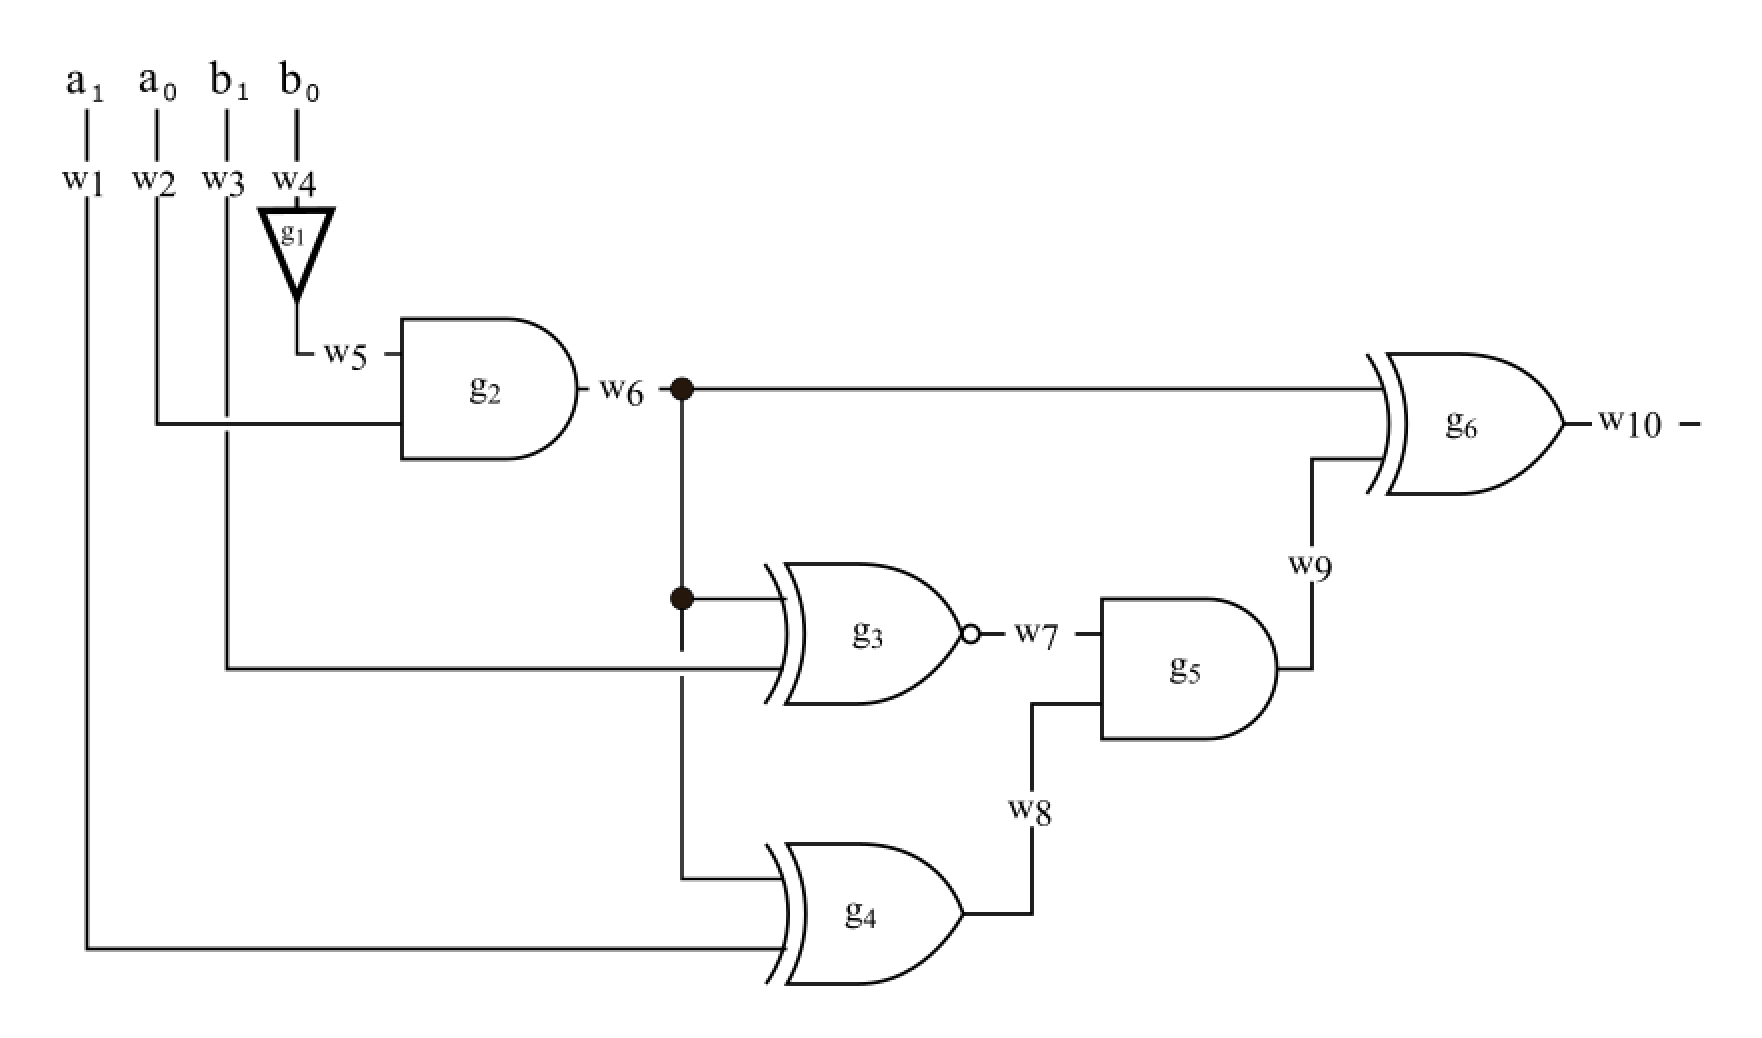
\includegraphics[scale=0.3]{Chapter_TechnicalOverview/booleanCircuit.png}

        \caption{Boolean circuit of the Millionaires' Problem. Optimized circuit according to the construction in \cite{Kolesnikov2009}.}
        \label{fig:boolean}
    \end{figure}
    
    In this case, the circuit contains one NOT gate ($g_1$), two AND gates ($g_2$, and $g_5$), two XOR gate ($g_4$ and $g_6$), one XNOR gate ($g_3$) and four input wires ($w_1$ and $w_2$ belonging to Alice and $w_3$ and $w_4$ to Bob).
    
    \item \textit{Wire encryption:} Alice uses a random number generator to generate two keys $k^0_i$ and $k^1_i$ for each wire $w_i$, $i\in\{1, ..., 10\}$. These keys correspond to the possible values ($0$ or $1$) on the wire. Note that this is done to prevent Bob from knowing the true value of the wires during the evaluation process.
    
    \item \textit{Gate encryption:} For every gate $g_l$ in the circuit with corresponding input wires $w_i$ and $w_j$ and output wire $w_s$, Alice creates the following table:

    \begin{center}
        \begin{tabular}{ |c| } 
        \hline
        $\mathsf{Enc}_{k_i^0}\left(\mathsf{Enc}_{k_j^0}\left(k_s^{g_l(0,0)}\right)\right)$ \\ 
        \hline
        $\mathsf{Enc}_{k_i^0}\left(\mathsf{Enc}_{k_j^1}\left(k_s^{g_l(0,1)}\right)\right)$ \\ 
        \hline
        $\mathsf{Enc}_{k_i^1}\left(\mathsf{Enc}_{k_j^0}\left(k_s^{g_l(1,0)}\right)\right)$ \\ 
        \hline
        $\mathsf{Enc}_{k_i^1}\left(\mathsf{Enc}_{k_j^1}\left(k_s^{g_l(1,1)}\right)\right)$ \\
        \hline
        \end{tabular}
    \end{center}
    
    where $g_l(a,b)$ is the output of gate $g_l$ for inputs $a, b\in \{0, 1\}$. So, we could think of each row as a locked box that requires two keys to be opened. If the two correct keys are used, it outputs the key corresponding to the desired output value given by $g_l$. After encrypting each gate, Alice permutes the rows of the corresponding table, otherwise, it would be easy to know the real value of the input keys. Then, she sends to Bob the garbled tables along with Alice's input keys.
    
    As an example, we can easily see that if we use input keys $k_i^0$ and $k_j^1$ (corresponding to real values $0$ and $1$), we would only be able to decipher the second row of the table, $\mathsf{Enc}_{k_i^0}(\mathsf{Enc}_{k_j^1}(k_s^{g_l(0,1)}))$, and get $k_s^{g_l(0,1)}$.
    
    \item \textit{Oblivious Transfer:} At this stage of the protocol, the evaluator Bob knows the garbled circuit and Alice's input keys but he does not know the keys corresponding to his real inputs. However, since Bob wants to keep his input value private he cannot directly ask for those keys. At this point, the OT functionality enables the evaluator to receive his input keys without compromising neither the evaluator's nor garbler's security. In fact, for every input wire, both parties perform an OT where Alice plays the role of the sender and Bob plays the role of the receiver. 
    
    Let us assume Alice's input keys to be $k_1^0$ and $k_2^1$ (corresponding to the real value  $01$) and Bob's input bits to be $11$. This means that Bob must use the respective input keys ($k_3^1$ and $k_4^1$) in order to correctly evaluate the circuit. So, they will execute two OT protocols where:
    
    \begin{itemize}
        \item Alice inputs: $(k_3^0, k_3^1)$ and $(k_4^0, k_4^1)$;
        \item Bob inputs: $b_1 = 1$ and $b_2 = 1$.
    \end{itemize}
    
    \item \textit{Evaluation:} Once the evaluator has all the necessary elements, he can proceed with the circuit evaluation. In this step, he simply has to decipher the correct rows of the garbled tables sent by Alice with the corresponding keys. Since the rows of the tables are shuffled, the evaluator does not know which row is the correct one. This small issue can be solved by simple techniques (Point-and-Permute or encryption with a certain number of $0$ padded) which, for the sake of brevity, we will not explore here. At the end of the evaluation, the evaluator receives the key that corresponds to the result. Finally, the evaluator sends the resulting key to the garbler and the garbler tells him the final bit.
    
    According to our Millionaires' problem, the evaluation yields the following results for $a = 01$ and $b = 11$: $g_1(k_4^1) = k_5^0$, $g_2(k_5^0, k_2^1) = k_6^0$, $g_3(k_6^0, k_3^1) = k_7^0$, $g_4(k_6^0, k_1^0) = k_8^1$, $g_5(k_7^0, k_8^1) = k_9^0$, $g_6(k_6^0, k_9^0) = k_{10}^0$. Actually, the desired result is $0$.
    
\end{enumerate}


The Yao protocol has its security based on two main building blocks: garbled circuits and oblivious transfer. Although garbled circuits can be generated with symmetric encryption (i.e. using double AES encryption), OT protocols cannot be classically achieved with symmetric cryptography alone \citep{IR89}. Thus, it is crucial to find efficient protocols for a quantum-resistant OT.

%Lindell and Pinkas presented a simulation-based proof that is based on the fact that 
%LP09


%Description
%
%Optimizations
%
%Security
%
%Generalizations of Yao: GMW, BMR

\subsection{Secret sharing approach}

The secret sharing approach was initiated by two concurrent works, known as BGW \cite{BGW88} and CCD \cite{CCD88}. This approach does not generate an ``encrypted" version of the circuit. Instead, the parties use some secret sharing scheme in order to evaluate the circuit. In this approach we use simple operations (addition and multiplication) but the communication rounds will depend on the size of circuit being evaluated. We start by defining an important primitive for secret sharing based protocols: oblivious linear evaluation.

\subsubsection{Oblivious linear evaluation}

Oblivious linear evaluation (OLE) can be seen as a generalization of oblivious transfer (OT) \cite{Rabin81}. OT has been shown to be complete for secure multi-party computation \cite{K88}, i.e., any such task, including OLE, can be achieved given an OT implementation. A compelling reason to study OLE protocols is that they can serve as building blocks for the secure evaluation of arithmetic circuits \cite{AIK11,DKMQ12,GNN17,DGNBNT17}, just like OT allows the secure evaluation of boolean circuits \cite{GMW87}. Specifically, OLE can be used to generate multiplication triples which are the basic tool for securely computing multiplication gates \cite{DGNBNT17}. Besides that, OLE has applications in more tasks for two-party secure computation  \cite{IPS09,ADINZ17,BCGI18,HIMV19,CDIKLOV19} and private set intersection \cite{GN19}.


\begin{figure}[h!]
\centering
\begin{tcolorbox}[enhanced, 
                        frame hidden,
                        ]
                        
    \centerline{$\mathcal{F}_{\textbf{OLE}}$ \textbf{functionality}}
            
    \
    
    \begin{itemize}
    		\item \textbf{Input phase:} Alice sends $(a,b)\in\mathbb{Z}_d^2$ (two field elements) to $\mathcal{F}_{\textbf{OLE}}$ and Bob sends $x\in\mathbb{Z}_d$ to $\mathcal{F}_{\textbf{OLE}}$.
    		\item \textbf{Output phase:} Alice receives nothing $\bot$ from the functionality and Bob receives $f(x):= ax + b$.
    \end{itemize}
    
\end{tcolorbox} 
    \caption{OLE functionality.}
    \label{fig:OLE_functionality}
\end{figure}

The OLE functionality specification is presented in Figure~\ref{fig:OLE_functionality}. Similarly, we have that OLE must satisfy the following security requirements:

\begin{itemize}
	\item Concealing: Alices knows nothing about Bob's field element $x$.
	\item Obliviousness: Bob knows nothing about the function $f()$ other than its evaluation at $x$, i.e. $f(x)$.
\end{itemize}

We can also generalize the OLE functionality to a vectorized version. The vector OLE (VOLE) functionality is presented in Figure~\ref{fig:VOLE_functionality}. Note that Bob only inputs one field element $x$ and Alice inputs two vectors. 


\begin{figure}[h!]
\centering
\begin{tcolorbox}[enhanced, 
                        frame hidden,
                        ]
                        
    \centerline{$\mathcal{F}_{\textbf{VOLE}}$ \textbf{functionality}}
            
    \
    
    \begin{itemize}
    		\item \textbf{Input phase:} Alice sends $(\bm{a},\bm{b})\in\mathbb{Z}_d^{2n}$ (two vectors of field elements) to $\mathcal{F}_{\textbf{VOLE}}$ and Bob sends only $x\in\mathbb{Z}_d$ to $\mathcal{F}_{\textbf{VOLE}}$.
    		\item \textbf{Output phase:} Alice receives nothing $\bot$ from the functionality and Bob receives $\bm{f}(x):= \bm{a}x + \bm{b}$.
    \end{itemize}
    
\end{tcolorbox} 
    \caption{VOLE functionality.}
    \label{fig:VOLE_functionality}
\end{figure}


\subsubsection{Basic operations}

To highlight the importance of OLE in secret sharing based SMC protocols, we go through a passively secure protocol \cite{Evans2018}. We consider the two party case (Alice and Bob) where the parties own additive shares of the secret. So, for some secret value $x$, Alice owns $x_A$, Bob owns $x_B$ and $x = x_A + x_B$. The operations used in the protocol according to the circuit are as follows:

\begin{itemize}
	\item \textbf{Input}. For Alice to secret share her input value $x$, she randomly chooses $x_B$ and sends it to Bob. Alice defines $x_A$ as $x_A = x - x_B$;
	\item \textbf{Addition}. There are two scenarios to consider:
	\begin{itemize}
		\item \textbf{Scalar}. For Alice and Bob to add a scalar to a secret $x$ ($z = a + x$), Alice computes $z_A = a + x_A$ and Bob sets $z_B = x_B$.
		\item \textbf{Shares}. For Alice and Bob to add secrets $x$ and $y$ ($z = x+y$), they individually add their corresponding shares, i.e. $z_A = x_A + y_A$ and $z_B = x_B + y_B$.
	\end{itemize}
	\item \textbf{Multiplication}. There are two scenarios to consider:
		\begin{itemize}
		\item \textbf{Scalar}. For Alice and Bob to multiply a secret by a scalar $x$ ($z = a \cdot x$), Alice computes $z_A = a \cdot x_A$ and Bob computes $z_B = a \cdot x_B$.
		\item \textbf{Shares}. Observe that, for Alice and Bob to multiply secrets $x$ and $y$ ($z = x\cdot y$), they require some sort of communication to compute cross terms:
		
		\begin{eqnarray}
		x\cdot y &=& (x_A + x_B)\cdot (y_A + y_B)\\
		&=& x_A\cdot y_A + x_A\cdot y_B + x_B \cdot y_A + x_B\cdot y_B
		\end{eqnarray}
		
		At this point, Alice and Bob can execute two OLE s to secret share the cross terms $x_A\cdot y_B$ and $x_B \cdot y_A$. Indeed, if Alice inputs $(x_A, - s_A)$ and $(y_A, - s'_A)$ for random values $s_A, s'_A$ and Bob inputs $y_B$ and $x_B$, Bob will output $s_B = x_A \cdot y_B - s_A$ and $s'_B = y_A \cdot x_B - s'_A$. Thus, we have that $s_A + s_B = x_A \cdot y_B$ and $s'_A + s'_B = y_A \cdot x_B$. So, Alice share is $z_A = x_A\cdot y_A + s_A + s'_A$ and Bob share is $z_B =  s_B + s'_B + x_B\cdot y_B$.  
	\end{itemize}
	\item \textbf{Output}. For Alice to receive the output value $x$ of some output wire, Bob simply sends $x_B$ to Alice. Alice outputs $x = x_A + x_B$.
\end{itemize}


%\bibliography{bibforthesis}
%\bibliographystyle{unsrt}
%\end{document}
